\documentclass[../../main/main.tex]{subfiles}
\begin{document}
\section{Appendix: Proof of Nash Equilibrium}
\label{app:nash_equilibrium}

\begin{customproof}
    To show that this is a Nash equilibrium, we need to show that no player can improve their payoff by unilaterally deviating from the strategy profile.
    
    In the proof, we assume that all of the constraints outlined in the previous section are satisfied. The solution was obtained by solving for $c(s)$ in terms of $x_2$, then using this to solve for $v(s)$, and finally solving for $b(s)$ up to a constant of integration. The resulting system of 7 equations in 7 unknowns was solved symbolically using Mathematica and simplified by finding common subexpressions $A_0, A_1, A_2, A_3, A_4, A_5$. The full Mathematica script is available in Appendix \ref{app:ma}.

    \begin{enumerate}
        \item \textbf{Caller's Deviation:}
            Fix the bet size $s$ and consider the caller's payoff from either calling or folding for each hand strength $y$. 

            \begin{align*}
                \mathbb{E}[\text{call} | y, s] &= \mathbb{P}[x < y | s](1+s) + \mathbb{P}[x \geq y | s](-s) \\
                \mathbb{E}[\text{fold} | y, s] &= 0 \\
            \end{align*}
            
            From section \ref{subsec:caller_indifference}, we know that the expected value of a call is exactly 0 for $y = c(s)$ (by design). The expected value of calling is weakly increasing in $y$, so it must be weakly greater than 0 for $y > c(s)$ and weakly less than 0 for $y < c(s)$. 

            \begin{figure}[h]
                \centering
                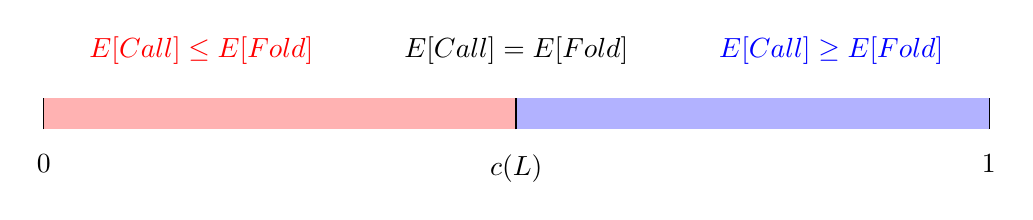
\begin{tikzpicture}[scale=4]
                    % Number line from 0 to 1
                    \draw[thick] (0,0) -- (3,0);
                    
                    % Tick marks at 0 and 1
                    \draw[thick] (0, -0.05) -- (0, 0.05);
                    \draw[thick] (3, -0.05) -- (3, 0.05);
                    
                    % Endpoint labels
                    \node[below] at (0, -0.1) {$0$};
                    \node[below] at (3, -0.1) {$1$};
                
                    
                    % Left segment (Fold) - red
                    \fill[red!30] (0, -0.05) rectangle (1.5, 0.05);
                    
                    % Right segment (Call) - teal/green
                    \fill[blue!30] (1.5, -0.05) rectangle (3, 0.05);
                    
                    % Threshold point c(L)
                    \draw[thick, black] (1.5, -0.05) -- (1.5, 0.05);
                    \node[below] at (1.5, -0.1) {$c(L)$};
                    
                    % Expected value conditions above
                    \node[red] at (0.5, 0.2) {$E[\text{Call}] \leq E[\text{Fold}]$};
                    \node[black] at (1.5, 0.2) {$E[\text{Call}] = E[\text{Fold}]$};
                    \node[blue] at (2.5, 0.2) {$E[\text{Call}] \geq E[\text{Fold}]$};
                    
                \end{tikzpicture}
                \caption{Caller's decision threshold $c(L)$. At hand strength of exactly $c(L)$, the caller is indifferent between calling and folding. Since the value of calling weakly increases with $y$, it must be weakly greater than 0 for $y > c(L)$ and weakly less than 0 for $y < c(L)$. Folding always has value 0.}
                \label{fig:caller_threshold}
            \end{figure}

            This proves that calling is weakly better than folding for all $y > c(s)$, and that folding is weakly better than calling for all $y < c(s)$, so the caller cannot improve their payoff by deviating from the strategy profile.  

        \item \textbf{Bettor's Deviation:}
            We need to consider a few cases.
            \begin{enumerate}
                \item $x < c(s)$:
                    These are hands and bet sizes for which the caller will call with only stronger hands (potential bluffs). The expected value of betting here is
                    \begin{align*}
                        \mathbb{E}[\text{bet } s | x] & = \mathbb{P}[\text{call with worse}] \cdot (1+s) - \mathbb{P}[\text{call with better}] \cdot s + \mathbb{P}[\text{fold}] \cdot 1 \\
                        & = 0 - (1-c(s)) \cdot (s) + c(s) \\
                        & = c(s) - (1-c(s)) \cdot s \\
                        & = x_2,
                    \end{align*}
                    with the last line coming from equation \ref{eq:bluffindiff}. The value of checking is always
                    \begin{align*}
                        \mathbb{E}[\text{check} | x] &= x.
                    \end{align*}
                    This means that (by design), the bettor is indifferent between checking and betting any amount at $x=x_2$. Importantly, the value of betting is independent of the hand strength $x$ while the value of checking is strictly increasing in $x$, so checking must be preferable for $x_2 < x < c(L)$ and betting must be preferable for $x < x_2$, which is exactly what our strategy profile does.
                    Because the value of bluffing is simply $x_2$ no matter the bet size or hand strength, we also know that the bettor cannot improve their payoff by bluffing with different bet sizes.
                \item $c(s) \leq x < x_3$:
                    These are hands and bet sizes for which the caller will at least sometimes call with weaker hands (potential value bets), but where the optimal strategy still checks. The expected value of betting here is
                    \begin{align*}
                        \mathbb{E}[\text{bet } s | x] & = \mathbb{P}[\text{call with worse}] \cdot (1+s) - \mathbb{P}[\text{call with better}] \cdot s + \mathbb{P}[\text{fold}] \cdot 1 \\
                        & = (x-c(s))(1+s) - (1-x) \cdot (s) + c(s) \\
                        & = s(2x - c(s) - 1) + x,
                    \end{align*}
                    while that of checking is 
                    \begin{align*}
                        \mathbb{E}[\text{check} | x] &= x.
                    \end{align*}
                    We know from \ref{eq:valueindiff} that
                    \begin{align*}
                        (x_3-c(L)) \cdot (1+L) - (1-x_3) \cdot (L) + c(L) & = x_3 \\
                        2x_3 - c(L) - 1 & = 0 \\
                    \end{align*}
                    Using our inequality $c(s) \leq x < x_3$ and the fact that $c(L)$ is the minimum of $c(s)$, we get
                    \begin{align*}
                        2x_3 - c(L) - 1 & = 0 \\
                        2x - c(s) - 1 & \leq 0.
                    \end{align*}
                    Substituting this into the expected value of betting, we get
                    \begin{align*}
                        \mathbb{E}[\text{bet } s | x] & = s(2x - c(s) - 1) + x \\
                        & \leq s \cdot 0 + x \\
                        & = x \\
                        &= \mathbb{E}[\text{check} | x].
                    \end{align*}
                    So no value can be gained by deviating from checking here.
                \item $x_3 \leq x < x_4$:
                    These are value bets where the bettor should bet the minimum. We need to show that the bettor cannot improve their payoff by either checking or by betting more.

                    The expected value of betting the minimum is
                    \begin{align*}
                        \mathbb{E}[\text{bet } L | x] & = L(2x - c(L) - 1) + x. 
                    \end{align*}
                    Again, we can use \ref{eq:valueindiff} to get 
                    \begin{align*}
                        2x_3 - c(L) - 1 & = 0 \\
                        2x - c(L) - 1 & \geq 0,
                    \end{align*}
                    since $x \geq x_3$. Substituting like before,
                    \begin{align*}
                        \mathbb{E}[\text{bet } L | x] & = L(2x - c(L) - 1) + x \\
                        & \geq L \cdot 0 + x \\
                        & = x \\
                        &= \mathbb{E}[\text{check} | x].
                    \end{align*}
                    So no value can be gained by deviating from betting to checking.

                    What about betting more? To show that this cannot improve the bettor's payoff, we show that the expected value of betting is weakly decreasing in $s$ for $x < x_4$, and must therefore be maximized at the lowest possible bet of $L$. 
                    
                    \begin{align*}
                        \frac{d}{ds} \mathbb{E}[\text{bet } s | x] & = -s c'(s) - c(s) + 2x - 1
                    \end{align*}
                    We know from \ref{eq:valueoptimality} that this equals $0$ when $x=v(s)$. We also know that $v(s)$ is at least $x_4$ for all $s \in [L, U]$, so $x < x_4 \leq v(s)$ for any such $s$. This means that
                    \begin{align*}
                        \frac{d}{ds} \mathbb{E}[\text{bet } s | x] & = -s c'(s) - c(s) + 2x - 1 \\
                        & \leq -s c'(s) - c(s) + 2x_4 - 1 \\
                        & = 0
                    \end{align*}
                    for any $s \in [L, U]$. Therefore, the expected value of betting is decreasing in $s$ for $x < x_4$, and must therefore be maximized at the lowest possible bet of $L$, so the bettor cannot improve their payoff by betting more.
                \item $x_4 \leq x < x_5$:
                    These are value bets where the bettor should bet an intermediate amount between $L$ and $U$. We need to show that the bettor cannot improve their payoff by either checking, betting less, or by betting more.

                    Rather than showing that checking is inferior to the optimal bet size, we show that checking is inferior to betting the minimum, which we will later show is inferior to the optimal bet size. Like the previous cases, the expected value of betting the minimum is
                    \begin{align*}
                        \mathbb{E}[\text{bet } L | x] & = L(2x - c(L) - 1) + x. 
                    \end{align*}
                    Like before, we know that $2x - c(L) - 1 \geq 0$ for $x \geq x_3$ (and in this case, $x \geq x_4 \geq x_3$). This means that
                    \begin{align*}
                        \mathbb{E}[\text{bet } L | x] & = L(2x - c(L) - 1) + x \\
                        & \geq L \cdot 0 + x \\
                        & = x \\
                        &= \mathbb{E}[\text{check} | x].
                    \end{align*}
                    So betting the minimum is at least as good as checking.

                    Now we show that betting any amount other than $v^{-1}(x)$ cannot gain value.
                    Let's again consider the derivative of the expected value with respect to $s$.
                    \begin{align*}
                        \frac{d}{ds} \mathbb{E}[\text{bet } s | x] & = -s c'(s) - c(s) + 2x - 1
                    \end{align*}
                    We know from \ref{eq:valueoptimality} that this is equal to $0$ when $x = v(s)$:
                    \begin{align*}
                        -s c'(s) - c(s) + 2v(s) - 1 &= 0.
                    \end{align*} 
                    This derivative is clearly an increasing function of $x$, so for $x < v(s)$, the expected value is decreasing in $s$. But since $v$ is an increasing function, $x < v(s)$ is equivalent to $v^{-1}(x) < s$ (essentially, our bet size is too large for the hand strength).
                    
                    This should make sense - when our bet size is too large for the hand strength, the expected value of that bet is decreasing in the bet size, so smaller bets are more profitable. We can show the same for bets too small: when $x > v(s)$, the expected value is increasing in $s$. This is equivalent to saying that $v^{-1}(x) > s$, or our bet size is too small for the hand strength, so larger bets are more profitable. 
                    
                    We have shown that the expected value of betting is increasing for $s < v^{-1}(x)$, equal to $0$ at $s = v^{-1}(x)$, and decreasing for $s > v^{-1}(x)$, so the expected value of betting is maximized at $s = v^{-1}(x)$. This means that the bettor cannot improve their payoff by deviating from this bet size. In particular, they cannot benefit by betting the minimum, which in turn proves that they cannot benefit by checking, as we showed above.
                \item $x_5 \leq x \leq 1$:
                    These are value bets where the bettor should bet the maximum. We need to show that the bettor cannot improve their payoff by either checking or betting less.

                    The expected value of betting the maximum is
                    \begin{align*}
                        \mathbb{E}[\text{bet } U | x] & = U(2x - c(U) - 1) + x. 
                    \end{align*}
                    Plugging $s=U$, $x=v(U)=x_5$ into \ref{eq:valueoptimality}, we get
                    \begin{align*}
                        -U c'(U) - c(U) + 2x_5 - 1 &= 0.
                    \end{align*}
                    What happens when $x > x_5$? This expression must be greater than $0$, meaning the expected value of betting is increasing in $s$ for $x > x_5$. If it is always increasing in $s$ for such $x$, then it must be maximized at the largest possible bet of $U$, so the bettor cannot improve their payoff by betting less.

                    We can use the exact same logic as the previous case to show that checking cannot improve the payoff either.
                    
            \end{enumerate}
    \end{enumerate}
\end{customproof}


\end{document}
